\documentclass[10pt,a4paper]{article}
\usepackage[UTF8]{ctex}
\usepackage{amsmath}
\usepackage[linesnumbered,ruled,vlined]{algorithm2e}
\usepackage{amssymb}
\usepackage{graphics}
\usepackage{graphicx}
\usepackage{fontspec}
\usepackage[top=2cm, bottom=2cm, left=2cm, right=2cm]{geometry} 
\usepackage{listings}
\usepackage{color}
\usepackage{subcaption}
\usepackage{booktabs}
\usepackage{array}
\usepackage{mathtools}
\usepackage{siunitx}
\usepackage[colorlinks=true, linkcolor=red, citecolor=red, urlcolor=red]{hyperref}
\definecolor{dkgreen}{rgb}{0,0.6,0}
\definecolor{gray}{rgb}{0.5,0.5,0.5}
\definecolor{mauve}{rgb}{0.58,0,0.82}


\title{最优化大作业上机报告}
\author{沙柯岑 2200010611}
\date{2024年12月13日}
\begin{document}
	\maketitle
	\tableofcontents
	\newpage
\section{问题描述}
\indent 考虑以下分组LASSO最优化问题
\begin{equation}
	\min_{x\in \mathbb{R}^{n\times l}}\frac{1}{2}\|Ax-b\|_{F}^{2}+\mu\|x\|_{1,2},
\end{equation}
这里$A\in \mathbb{R}^{m\times n}$, $b\in \mathbb{R}^{n\times l}$, $\mu>0$是给定的常数,并且
$$\|x\|_{1,2}=\sum\limits_{i=1}^{n}\|x(i,1:l)\|_{2}.$$
\begin{enumerate}
	\item 分别用cvx调用gurobi和mosek求解器求解上述最优化问题.
	\item 首先写出(1)的等价模型,使得可以被mosek和gurobi直接求解,并实施相应的代码.
	\item 分别按照以下方法求解最优化问题(1):
	\begin{enumerate}
		\item 对原问题使用次梯度法;
		\item 对原问题使用光滑化的梯度法;
		\item 对原问题使用临近点算法;
		\item 对原问题使用加速的临近点算法;
		\item 对对偶问题使用增广拉格朗日函数法;
		\item 对对偶问题使用交替方向乘子法;
		\item 对原问题结合线性化技巧使用交替方向乘子法.
	\end{enumerate}
\end{enumerate}
\section{问题分析及相应结果}
\indent 为保证结果可以复现,以下问题所有地结果均在一固定种子下生成,在代码开头将种子设定为“24847563”,即可得到相应的结果.
\subsection{问题1}
\indent 直接将原问题的形式在cvx中等价地表达出来即可,以下是两个不同的求解器得到的结果,数值结果保留5位有效数字\footnote{后面的表格中的数据也按照这个标准.},时间以秒为单位保留两位小数\footnote{8,9秒的时间是不必要的,后来进行优化减少了时间(见总表),事后发现是建立模型时不够简洁导致的}.从\hyperref[2]{表1}可以看出两个求解器的效果相差不大.
\begin{table}[h]
	\centering
	\begin{tabular}{|c|c|c|c|c|c|c|}
		\hline
		solver& Fval  &Time&Sparisity& Errfun\_exact &Err-to-cvx-mosek&Err-to-cvx-gurobi\\
		\hline
		cvx-mosek&6.0715e-01&8.42&0.110&4.1480e-05&0&2.5553e-07\\
		\hline
		cvx-gurobi&6.0715e-01&9.96&0.110&4.1312e-05&2.5553e-07&0\\
		\hline
	\end{tabular}
	\caption{用cvx求解的结果}
	\label{2}
\end{table}
\subsection{问题2}
\indent 对于mosek求解器,将原问题转化为二次锥规划问题如下:
\begin{equation}
	\begin{alignedat}{2}
		&\min_{x\in \mathbb{R}^{n\times l}, t\in \mathbb{R}, s\in\mathbb{R}^{n}} &\quad& \frac{t}{2}+\mu\cdot\mathbf{1}^{\top}s,\\
		&\qquad\quad\text{s.t.}\phantom{{}_{x\in \mathbb{R}^{n\times l}, t\in \mathbb{R}, s\in\mathbb{R}^{n}}} & & \|x(i,1:l)\|_{2}\leq s(i),\qquad 1\leq i\leq n\\
		&&&\|Ax-b\|_{F}^{2}\leq t.
	\end{alignedat}
	\label{3}
\end{equation}
这里,$\mathbf{1}=(1,1,\cdots,1)^{\top}$,在实际写代码时,还需将最后一个旋转二次锥约束转化为标准的二次锥约束.根据mosek语法,我们创建了$nl+n+1$个变量分别表示$x(i,j)$, $s(i)$以及$t$. Mosek要求所有二次锥约束都写成标准形式
$$Fx+g\in \mathcal{S},$$
其中$\mathcal{S}=\{(u,v)^{\top}\in\mathbb{R}^{k+1}|\|u\|_{2}\leq v\}$,对\hyperref[3]{(2)}中的$n+1$个锥约束写出相应的$F,g$再将它们组合在一起,即可使用mosek对原问题进行求解(具体可参见相应代码文件).\\
\indent 对于gurobi求解器,需要将问题转化为带二次约束的二次规划的形式如下:
\begin{equation}
	\begin{alignedat}{2}
		&\min_{u\in \mathbb{R}^{m\times l}, x\in \mathbb{R}^{n\times l}, s\in\mathbb{R}^{n}} &\quad& \frac{1}{2}\|u\|_{F}^{2}+\mu\cdot\mathbf{1}^{\top}s,\\
		&\qquad\quad\text{s.t.}\phantom{{}_{x\in \mathbb{R}^{n\times l}, t\in \mathbb{R}, s\in\mathbb{R}^{n}}} & & x(i,1:l)x(i,1:l)^{\top}-s(i)^{2}\leq 0,\qquad 1\leq i\leq n\\
		&&&s(i)\geq 0,\\
		&&&Ax-u=-b.
	\end{alignedat}
	\label{4}
\end{equation}
这里,$\mathbf{1}=(1,1,\cdots,1)^{\top}$.类似mosek,我们需要创建$(m+n)l+n$个变量分别表示$u$, $x$, $s$.在实际写代码时,根据gurobi语法,需要分别写出一、二次项部分$F$, $Q\in  \mathbb{R}^{[(m+n)l+n]\times [(m+n)l+n]}$,变量范围$lb$,$ub\in \mathbb{R}^{(m+n)l+n}$(分别表示各变量的下界和上界),以及\hyperref[4]{(3)}中的$n$个二次约束,完成这些内容即可用gurobi对原问题进行求解(具体可参见相应代码文件).\\
\indent 以下是建立上述模型后分别直接用mosek和gurobi求解器得到的结果.从\hyperref[5]{表2}可以看出我们建立的gurobi模型求解效果相比cvx-mosek、cvx-gurobi、mosek都要差一些\footnote{gurobi的版本会影响结果,用gurobi 11.0.3得到的结果会略好一些,该实验采用的是gurobi 12.0.0版本.},尤其是稀疏性效果不佳,因此仍然有改进的空间.当然,因为问题\hyperref[4]{(3)}可以写成其他的等价形式,也可以用gurobi语法实现,比如:
\begin{equation}
	\begin{alignedat}{2}
		&\min_{x\in \mathbb{R}^{n\times l}, s\in\mathbb{R}^{n},t\in \mathbb{R}} &\quad& \frac{t}{2}+\mu\cdot\mathbf{1}^{\top}s,\\
		&\qquad\quad\text{s.t.}\phantom{{}_{x\in \mathbb{R}^{n\times l}, t\in \mathbb{R}, s\in\mathbb{R}^{n}}} & & x(i,1:l)x(i,1:l)^{\top}-s(i)^{2}\leq 0,\qquad 1\leq i\leq n\\
		\
		&&&s(i)\geq 0,\\
		&&&\|Ax-b\|_{F}^{2}\leq t.
	\end{alignedat}
	\label{6}
\end{equation}
或者
\begin{equation}
	\begin{alignedat}{2}
		&\min_{x\in \mathbb{R}^{n\times l}, s\in\mathbb{R}^{n}} &\quad& \frac{1}{2}\sum\limits_{i=1}^{l}(x_{i}^{\top}A^{\top}Ax_{i}-2b_{i}^{\top}x_{i}+b_{i}^{\top}b_{i})+\mu\cdot\mathbf{1}^{\top}s,\\
		&\qquad\quad\text{s.t.}\phantom{{}_{x\in \mathbb{R}^{n\times l}, t\in \mathbb{R}, s\in\mathbb{R}^{n}}} & & x(i,1:l)x(i,1:l)^{\top}-s(i)^{2}\leq 0,\qquad 1\leq i\leq n\\
		&&&s(i)\geq 0.\\
	\end{alignedat}
	\label{7}
\end{equation}
这里$x_{i}$表示$x$的第$i$列,$b_{i}$表示$b$的第$i$列.这两个模型求解的效果比\hyperref[4]{(3)}更差,甚至不能收敛到最优解,结果如\hyperref[8]{表3}所示,因此在使用gurobi求解器解二次规划问题时,应尽量简化目标函数二次型的形式,(比较\hyperref[4]{(3)}和\hyperref[6]{(4)}),优先选择线性约束而非二次约束(比较\hyperref[4]{(3)}和\hyperref[7]{(5)}).
\begin{table}[h]
	\centering
	\begin{tabular}{|c|c|c|c|c|c|c|c|}
		\hline
		solver& Fval&Iter  &Time&Sparisity& Errfun\_exact &Err-to-cvx-mosek&Err-to-cvx-gurobi\\
		\hline
		mosek&6.0715e-01&11&0.79&0.110&4.1413e-05&1.0231e-07&1.6911e-07\\
		\hline
		gurobi&6.0715e-01&11&0.83&0.121&4.3251e-05&2.2605e-06&2.4753e-06\\
		\hline
	\end{tabular}
	\caption{直接用mosek和gurobi求解的结果}
	\label{5}
\end{table}
\begin{table}[h]
	\centering
	\begin{tabular}{|c|c|c|c|c|c|c|c|}
		\hline
		solver& Fval&Iter  &Time&Sparisity& Errfun\_exact &Err-to-cvx-mosek&Err-to-cvx-gurobi\\
		\hline
		gurobi(3)&6.0715e-01&11&0.83&0.121&4.3251e-05&2.2605e-06&2.4753e-06\\
		\hline
		gurobi(4)&6.8843e-01&30&2.07&0.992&2.9837e-03&2.9617e-03&2.9618e-03\\
		\hline
		gurobi(5)&6.0759e-01&15&0.92&0.274&5.1274e-05&1.1977e-05&1.2164e-05\\
		\hline
	
	\end{tabular}
	\caption{用不同的gurobi模型求解的结果}
	\label{8}
\end{table}
\subsection{问题3.(a)}
\indent 记目标函数为$f(x,\mu)$,则$f(x,\mu)$关于$x$的次梯度为(按每一行表示):
$$\partial f(x,\mu)(i,:)=(A^{\top}(Ax-b))(i,:)+
\begin{cases}
	\mu x(i,1:l)/\|x(i,1:l)\|_{2} & \text{if } x(i,1:l)\neq 0,\\
	\{\mu g\in \mathbb{R}^{1\times l}\||g\|_{2}\leq 1\} & \text{else.}
\end{cases}$$
我们采用次梯度法,并且结合BB步长、回退法线搜索、连续化策略完成对该问题的求解. 具体算法步骤如下:
\begin{algorithm}[H]
	\SetAlgoLined
	\KwIn{初始点$x_{0}$, $A$, $b$, $\mu$, 常数$L$,连续化参数$\rho>1$, $k\in \mathbb{N^{*}}$, $iter=0$, $f^{*}=\inf$.}
	\KwResult{返回最优解$x_{0}$,最小值$f^{*}$,迭代次数$iter$.}
	$v=\mu\times\rho^{k};$
	$x_{1}=x_{0}-\frac{1}{L}\partial f(x_{0},v)$\;
	
	\While{$ v\neq\mu \lor |f(x_{1},\mu)-f(x_{0},\mu)|\geq 10^{-10}$}{
		$s=x_{1}-x_{0}$, $y=\partial f(x_{1},v)-\partial f(x_{0},v)$, $g=\partial f(x_{1},v)$\;
		$\alpha_{BB}=\|s\|_{F}^{2}/\langle s,y\rangle $, $a=\max(\alpha_{BB},L)$\;
		
		\While{$a>\frac{1}{L}\land f(x_{1},v)-f(x_{1}-ag,v)<\frac{1}{2L}\|g\|_{F}^{2} $}
		{$a=a/2$\;
		}
		\While{$f(x_{1},v)-f(x_{1}-ag,v)<0$}
		{$a=a/2$\;
			\If{$a<10^{-15}$}{\textbf{break}}
		}
		$x_{0}=x_{1}$, $x_{1}=x_{1}-ag$, $iter=iter+1$, $f^{*}=\min(f^{*},f(x_{0},\mu))$\;
		\If{$v>\mu \land \|f(x_{0},v)-f(x_{1},v)\|\leq 10^{-5}\cdot v $}
		{$v=v/\rho$\;
		}
	}
	\KwOut {$x_{0}$, $iter$, $f^{*}$}
	\caption{次梯度法求解最优化问题(1)}
	\label{alg 1}
\end{algorithm}
在该算法中,我们先将$\mu$适当增大至$v$,对$f(x,v)$求解最优化问题,当求解到一定程度时适当减小$v$,直至$v=\mu$. 理论上不可微函数没有Lipchitz连续性,这里为了防止BB步长过大,设置的默认$L=\|A^{\top}A\|_{2}$\footnote{L的选取受梯度下降法的启发,当$\|x\|$不太小时,可以将$f$看成梯度$L-Lipchitz$连续的函数},为了防止BB步长过小,设置了最小步长$10^{-15}$.\\
\indent 此外,次梯度的选取也很重要,因为当$\|x(i,:)\|_{2}$过小时,次梯度$x(i,1:l)/\|x(i,1:l)\|_{2}$的误差会很大,因此需要设置一个阈值$\epsilon$, 当$\|x(i,:)\|_{2}\leq\epsilon$时,将其视为0\footnote{严格地说,应该是不用$ x(i,1:l)/\|x(i,1:l)\|_{2}$去计算,而是取一个$\|g\|_{2}\leq 1$,正如后文所示.},并且此时取对应的次梯度分量$\partial f(x,\mu)(i,:)=(A^{\top}(Ax-b))(i,:)+x(i,:)/\epsilon$,经过试验,取$\epsilon=10^{-6}$就能够得到较好的结果.\\
\indent 推荐的连续化参数为$\rho=5$, $k=5$.线搜索采用回退法,分为两个阶段,步长$>L$时,采用弱化的armijo准则($c_{1}=\frac{1}{2}$, 要求从$\frac{a}{2}$降至$\frac{1}{2L}$),步长$<L$时,只需保证每一次单调下降即可.\\
\indent 下面是次梯度下降法得到的结果图像,作为比较,还试验了不加BB步长和不加连续化策略的结果.在本例中,不加BB步长也能达到很好的效果,然而,在问题3(b)我们将看到BB步长的作用.此外,如果不用连续化技巧,算法需要约20万步才能收敛.
\begin{figure}[ht]
	\centering
	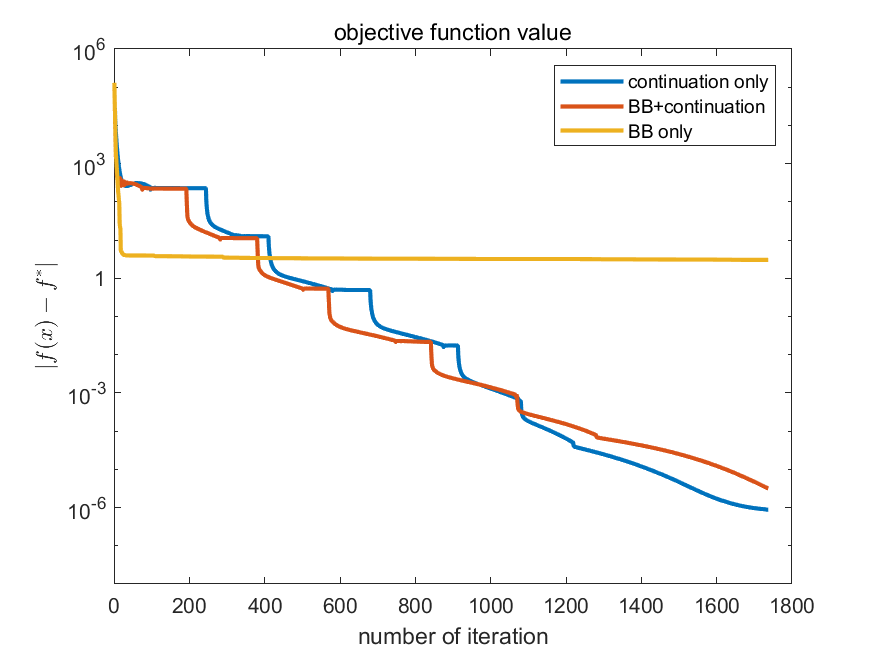
\includegraphics[width=0.5\textwidth]{figure.3(a).png}
	\caption{次梯度法求解得到的结果}
	\label{9}
\end{figure}
\subsection{问题3.(b)}
\indent 采用光滑化策略对SGD算法进行加速,我们采用huber光滑函数对$\|x(i,:)\|_{2}$光滑化, huber函数为
$$h_{u}(x)=\begin{cases}
	\frac{x^{2}}{2u} & \textbf{if }0\leq x\leq u,\\
	x-\frac{u}{2}  &\textbf{if }x\geq u.
\end{cases}
$$
光滑化后的函数为
$$f_{u}(x,\mu)=\frac{1}{2}\|Ax-b\|_{F}^{2}+\mu\sum\limits_{i=1}^{n}h_{u}(\|x(i,:)\|_{2}),$$
并且
$$
	|f_{u}(x,\mu)-f(x,\mu)|\leq \frac{\mu nu}{2}.
$$
容易证明,$h_{u}(x)$是梯度$\frac{1}{u}$-Lipchitz连续的,进而$f_{u}(x,\mu)$是梯度$(\|A^{\top}A\|_{2}+\frac{\mu\sqrt{n}}{u})$-Lipchitz连续的\footnote{实际中取$L=\|A^{\top}A\|_{2}+\frac{\mu}{u}$就可以达到很好的效果},因此可以用标准的梯度算法求解,也可以使用BB步长+线搜索的方法.如3(a)一样我们采用连续化策略,这里我们采取了一个小技巧,随着$u$的增大,光滑化函数的梯度Lipchitz常数也在增大,因此在降低$u$的同时可以同时降低$\mu$,保证在迭代初期Lipchitz常数不会增大,有较快的收敛速度.\\
\indent	下面是光滑化梯度下降法得到的结果图像,我们一共做了4组试验.由\hyperref[10]{图2}可以看出,BB步长在加速收敛起到关键作用,比连续化策略的作用更大,二者结合可以得到更快的收敛速度.
\begin{figure}[ht]
	\centering
	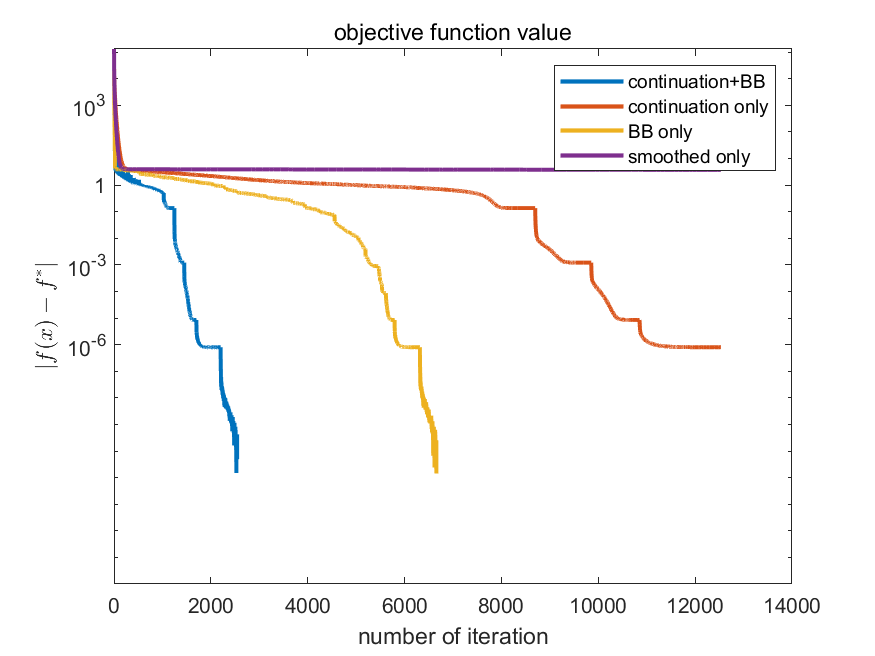
\includegraphics[width=0.5\textwidth]{figure.3(b).png}
	\caption{光滑化梯度法求解得到的结果}
	\label{10}
\end{figure}
尽管光滑化技巧所需要的迭代次数略多,但能够达到更好的精度,并且非光滑的次梯度算法结果受参数的影响很大,要想达到更高的精度需要相当多的迭代步数,\hyperref[11]{表4}是光滑化与非光滑结果的比对.
\begin{table}[h]
	\centering
	\begin{tabular}{|c|c|c|c|c|c|c|c|}
		\hline
		solver& Fval&Iter  &Time&Sparisity& Errfun\_exact &Err-to-cvx-mosek&Err-to-cvx-gurobi\\
		\hline
		non-smoothed&6.0715e-01&1983&0.51&0.113&4.5045e-05&4.0763e-06&4.2597e-06\\
		\hline
		smoothed&6.0715e-01&3325&0.70&0.110&4.1520e-05&1.9296e-07&2.3676e-07\\
		\hline
	\end{tabular}
	\caption{3(a)与3(b)结果对比}
	\label{11}
\end{table}
\subsection{问题3(c),3(d)}
记$f(x)=\frac{1}{2}\|Ax-b\|_{F}^{2}$, $h_{\mu}(x)=\mu \|x\|_{1,2}$,则$h_{\mu}(x)$的临近点算子表达式为(按行分量分别表示):
$$\text{prox}_{th_{\mu}}(y)(i,:)=\begin{cases}
	0&\text{if } \|y(i:)\|_{2}\leq t\mu,\\
	y(i,:)-t\mu\frac{y(i,:)}{\|y(i,:)\|_{2}} &\text{else.}
\end{cases}\qquad ,1\leq i\leq n
$$
记$L=\|A^{\top}A\|_{2}$,则$f(x)$是梯度$L-$Lipchitz连续的,从而可用标准的近似点梯度法求解,迭代格式如下:
$$\begin{aligned}
	&y_{k}=x_{k}-\frac{1}{L}\nabla f(x_{k});\\
	&x_{k+1}=\text{prox}_{\frac{1}{L}h_{\mu}}(y_{k}).
\end{aligned}$$
我们仍然想尝试用BB步长观察是否有加速效果,以及连续化策略的加速效果,方式类似\hyperref[alg 1]{算法1},问题3(d)采用的是FISTA加速算法以及连续化策略,如\hyperref[alg 2]{算法 2}所示:\\
\begin{algorithm}[H]
	\SetAlgoLined
	\KwIn{矩阵$A \in \mathbb{R}^{m\times n}$, 向量$b \in \mathbb{R}^l$, 参数$\mu$, 初始点$x_0$,常数$L$,连续化参数$\rho>1$, $N\in\mathbb{N^{*}}$.}
	\KwResult{返回最优解$x_{0}$,最小值$f^{*}$,迭代次数$iter$.}
	$iter = 0$; % 初始化计数器\;
	$k = 1$; % 初始化加速参数\;
	$v = \mu \times \rho^N$; % 初始化次梯度参数\;
	$x_1 = \text{prox}_{\frac{1}{L}h_{v}}\left(x_0 - \frac{1}{L} A^T (A x_0 - b), \frac{1}{L}\right)$; % 初始点通过近端算子更新\;
	
	\While{$v \geq \mu$}{
		$f^{*} = f(x_0)$; % 计算当前目标函数值\;
		$iter = iter + 1$; % 迭代计数器增加\;
		$k = k + 1$\; % 更新Nesterov加速度参数\;
		$y = x_1 + \frac{k-2}{k+1}(x_1 - x_0)$; % Nesterov加速度\;
		$x_0 = x_1$; % 更新旧点\;
		$x_1 = \text{prox}_{\frac{1}{L}h_{v}}\left(y - \frac{1}{L} A^T (A y - b), \frac{1}{L}\right)$; % 新点基于近端算子更新\;
		
		\If{$\|x_0 - x_1\|_F < 10^{-5} \land v > \mu$}{
			$v = v / \rho$; % 减小次梯度参数\;
			$k = 1$; % 重置加速参数\;
		}
		\If{$v == \mu \land \|x_0 - x_1\|_F < 10^{-8}$}{
			\textbf{break}; % 满足条件则跳出循环\;
		}
	}
	\KwOut {$x_0$, $iter$, $f^{*}$}
	\caption{使用FISTA加速临近点算法求解最优化问题}
	\label{alg 2}
\end{algorithm}
\hyperref[13]{图3}是采用近似点梯度法得到的数值结果,分为两组,一组包含连续化策略而另一组不包含.推荐的连续化参数为$\rho=10$, $N=5$, 可以看到,与光滑化方法不同,连续化策略在临近点算法的效果比BB方法更显著.相比于次梯度法和光滑化梯度法,临近点算法的收敛速度更快,精度也更高,\hyperref[14]{表5}是用临近点算法得到的性能指标(均使用连续化策略).
\begin{figure}[ht]
	\centering
	\begin{subfigure}[b]{0.45\textwidth}
	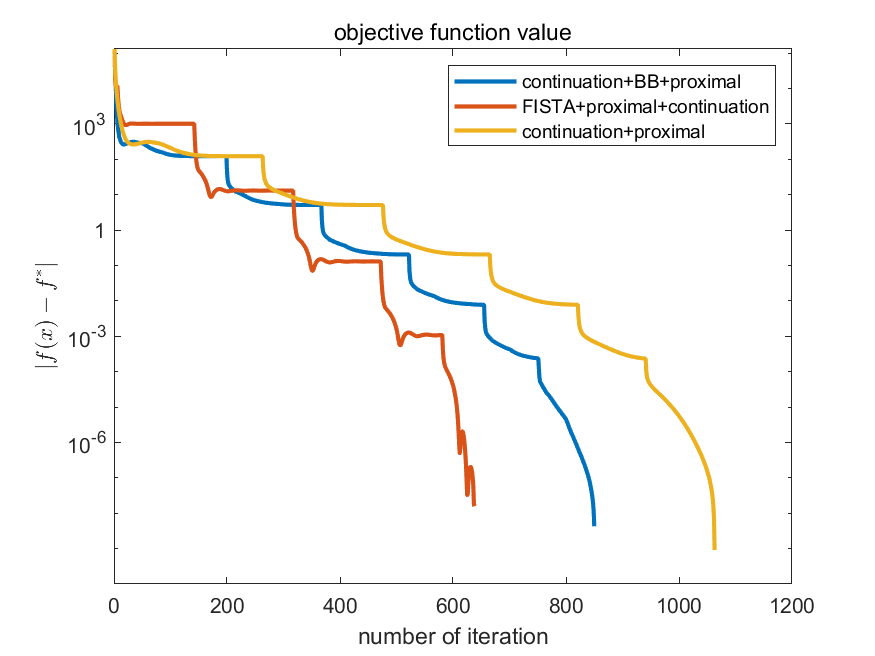
\includegraphics[width=\textwidth]{figure.3(c)&3(d).proximal1.png}
	\caption{带连续化技巧的临近点算法}
	\label{fig:sub1}
	\end{subfigure}
	\hfill
	\begin{subfigure}[b]{0.45\textwidth}
	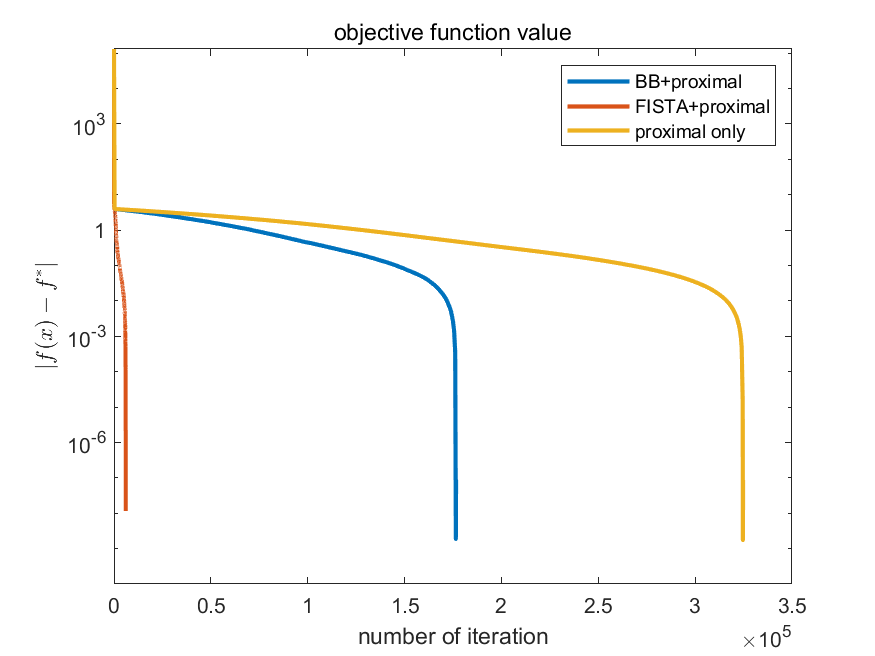
\includegraphics[width=\textwidth]{figure.3(c)&3(d).proximal2.png}
	\caption{不带连续化技巧的临近点算法}
	\label{fig:sub2}
	\end{subfigure}
	\caption{近似点算法求解得到的结果}
	\label{13}
\end{figure}
\begin{table}[h]
	\centering
	\begin{tabular}{|c|c|c|c|c|c|c|c|}
		\hline
		solver& Fval&Iter  &Time&Sparisity& Errfun\_exact &Err-to-cvx-mosek&Err-to-cvx-gurobi\\
		\hline
		proximal+BB&6.0715e-01&947&0.13&0.110&4.1329e-05&2.4914e-07&2.6723e-07\\
		\hline
		proximal+FISTA&6.0715e-01&841&0.04&0.110&4.1328e-05&2.4999e-07&2.5531e-08\\
		\hline
	\end{tabular}
	\caption{3(d)与3(e)的结果对比}
	\label{14}
\end{table}
\subsection{问题3(e)}
\indent 原问题的对偶问题是:
\begin{equation*}
\begin{aligned}
	&\min_{y\in\mathbb{R}^{m\times l}}  &\frac{1}{2}\|y\|_F^2 - \langle y, b\rangle,\\
	&\text{\quad\quad\, s.t.} &\|A^{\top}y\|_{1,2}\leq\mu.
\end{aligned}
\end{equation*}
为了让约束函数可微,我们改写为如下等价的优化问题:
\begin{equation*}
	\begin{aligned}
		&\min_{y\in\mathbb{R}^{m\times l},s\in\mathbb{R}^{n\times l}}  &&\frac{1}{2}\|y\|_F^2 - \langle y, b\rangle,\\
		&\text{\quad\quad\, s.t.} &&\|(A^{\top}y)_{i}\|^{2}\leq\mu^{2}.\qquad 1\leq i\leq n
	\end{aligned}
\end{equation*}
其中$(A^{\top}y)_{i}$表示矩阵$A^{\top}y$的第$i$行.约束是不等式约束,通过消元,可以得到如下增广拉格朗日函数:
$$L_{\sigma}(y,\lambda)=\frac{1}{2}\|y\|_F^2 - \langle y, b\rangle+\frac{\sigma}{2}\sum\limits_{i=1}^{n}(\max\{\frac{\lambda_{i}}{\sigma}+\|(A^{\top}y)_{i}\|_{2}^{2}-\mu^{2},0\}^{2}-\frac{\lambda_{i}^{2}}{\sigma^{2}}).
$$
记乘子更新函数为:
$$U_{i}(\sigma,y,\lambda)=\max\{\lambda_{i}+\sigma(\|(A^{\top}y)_{i}\|_{2}^{2}-\mu^{2}),0\},\quad 1\leq i\leq n$$
$$\vec{U}(\sigma,y,\lambda)=(U_{i}(\sigma,y,\lambda))^{\top}.$$
增广拉格朗日函数关于$y$的梯度为:
$$\nabla_{y}L_{\sigma}(y,\lambda)=y-b+2A\cdot diag(\vec{U}(\sigma,y,\lambda))\cdot A^{\top}y.$$
乘子更新公式为:
$$\lambda_{i}^{k+1}=U_{i}(\sigma_{k},y_{k+1},\lambda^{k})=\max\{\lambda_{i}^{k}+\sigma_{k}(\|(A^{\top}y_{k+1})_{i}\|_{2}^{2}-\mu^{2}),0\}.\quad 1\leq i\leq n$$
约束违反度为:
$$V(\sigma_{k},y_{k+1},\lambda^{k})=\frac{\|\vec{U}(\sigma_{k},y_{k+1},\lambda^{k})-\lambda^{k}\|_{2}}{\sigma_{k}}.$$
采用一般约束问题增广拉格朗日函数法算法如\hyperref[alg 3]{算法3}所示:\\
\begin{algorithm}[H]
	\SetAlgoLined
	\DontPrintSemicolon
	\KwIn{矩阵 $A$, 向量 $b$, 参数 $\mu$,罚因子增长率 $\rho$,初始罚因子$\sigma$,罚因子上限$M$,目标精度$\eta$,目标约束违反度 $\varepsilon$,初始精度$\eta_{0}$,初始约束违反度$\varepsilon_{0}$,衰减指数$\beta$}
	初始化 $\lambda^{0} = \mathbf{0}_{n\times 1}$, $y_{0} = \mathbf{0}_{m\times l}$, 外循环次数$k=0$\;
	\While{$V(\sigma_{k},y_{k},\lambda^{k}) > \varepsilon \lor \| \nabla L_{\sigma_{k}}(y_{k},\lambda^{k}) \|_\text{F} > \eta$}{
		\If{$\sigma > M$}{
			\textbf{break}
		}
		以初始点$y_{k}$用Nesterov加速算法求解最优化子问题$y_{k+1} =\text{argmin}_z L_\sigma(z,\lambda^{k})$ 使得 $\|\nabla_{y}L_{\sigma}(y_{k+1},\lambda)\|\leq\eta_{k}$\;
		
		\uIf{$V(\sigma_{k},y_{k},\lambda^{k}) \leq \varepsilon_{k}$}{
			\If{$V(\sigma_{k},y_{k},\lambda^{k})\leq \varepsilon_0 \land \| \nabla_{y} L_{{\sigma}_{k}}(y_{k},\lambda^{k}) \|_\text{F} \leq \eta_0$}{
					\textbf{break}
			}
			$\lambda^{k+1} = \vec{U}(\sigma_{k},y_{k+1},\lambda^{k})$\;
			$\varepsilon_{k+1} = \varepsilon_{k+1} / \rho$\;
			$\sigma_{k+1} =\sigma_{k}$\;
			$\eta_{k+1} = \eta_{k}$\;
		}\Else{
			$\sigma_{k+1} = \rho \cdot \sigma_{k}$\;
			$\eta_{k+1} = \eta_{k} / \rho^{\beta}$\;
			$\lambda^{k+1} =\lambda^{k}$\;
			$\varepsilon_{k+1} = \varepsilon_{k+1}$\;
		}
		$k=k+1$\;
	}
	\KwResult{极小点$y^*$, 乘子$\lambda_*$, 外循环次数$k$}
	\caption{增广拉格朗日乘子法用于对偶问题}
	\label{alg 3}

\end{algorithm}
算法中的Nesterov加速方法类似于\hyperref[alg 2]{算法2}的FISTA,只不过没有取临近点.推荐的参数是$\sigma_{0}=10^5$, $\rho=10$, $\beta=\lg 5$, $M=10^{7}$, $\varepsilon=10^{-7}$, $\eta=10^{-5}$, $\eta_{0}=\varepsilon_{0}=10^{-2}$.\\
\indent 除此以外,还设置了罚因子上限,经验表明,初始罚因子应取得比较大,相同的精度比约束违反度更难满足,因此精度上升的速度慢一些(由衰减指数$\beta$控制)得到的数值结果将在最后的总表中显示.
\subsection{问题3(f)}
原问题的对偶问题还可以写成
\begin{equation*}
	\begin{aligned}
		&\min_{y\in\mathbb{R}^{m\times l},s\in\mathbb{R}^{n\times l}}  &&\frac{1}{2}\|y\|_F^2 - \langle y, b\rangle,\\
		&\text{\quad\quad\, s.t.} &&A^{\top}y-s=0,\\
		&&&\|s\|_{1,2}\leq\mu.
	\end{aligned}
\end{equation*}
去掉不等式约束,令集合$\textbf{C}=\{s\in\mathbb{R}^{n\times l}|\|s\|_{1,2}\leq\mu\}$对偶问题还可以写成
\begin{equation*}
	\begin{aligned}
		&\min_{y\in\mathbb{R}^{m\times l},s\in\mathbb{R}^{n\times l}}  &&\frac{1}{2}\|y\|_F^2 - \langle y, b\rangle+\mathbf{1}_{\textbf{C}}(s),\\
		&\text{\quad\quad\, s.t.} &&A^{\top}y-s=0.\\
	\end{aligned}
\end{equation*}
问题化为这种形式即可使用交替方向乘子法.首先写出该问题的增广拉格朗日函数
$$L_{\sigma}(y,s,\lambda)=\frac{1}{2}\|y\|_F^2 - \langle y, b\rangle+\mathbf{1}_{\textbf{C}}(s)+\langle\lambda, A^{\top}y-s\rangle +\frac{\sigma}{2}\|A^{\top}y-s\|_{F}^{2}.$$
首先固定$s$,对$L_{\sigma}$关于$y$求极小值,这是关于$y$的二次函数,极小值有显式表达:
\begin{equation}
y^{*}=(I+\sigma AA^{\top})^{-1}(b+A\lambda+\sigma As).
\label{eq.6}
\end{equation}
然后固定所求的$y$,再对$L_{\sigma}$关于$s$求极小值,经过简单计算可知$s$也有显示表达\footnote{在实际写代码时不需要将每个分量写出来,这里只是为了表达方便和直观.}:
\begin{equation}
	s_{i}=\left( (A^{\top}y)_{i}+\frac{\lambda_{i}}{\sigma}\right) \min\{\frac	{\mu}{\|(A^{\top}y)_{i}+\frac{\lambda_{i}}{\sigma}\|},1\},\quad 1\leq i\leq n
\label{eq.7}
\end{equation}
其中$s_{i}$表示矩阵变量$s$的第$i$行.在内循环中求解\eqref{eq.6}时,先求出$I+\sigma AA^{\top}$的Cholesky分解再求出相应的$y^*$,得到如下ADMM算法,并且根据原始可行性条件和对偶可行性条件违反度的相对情况动态调节罚因子:\\
\begin{algorithm}[H]
	\SetAlgoLined
	\DontPrintSemicolon
	\KwIn{矩阵 $A$, 向量 $b$, 参数 $\mu$, 罚因子变化率 $\rho$,初始罚因子 $\sigma$,协调率 $\eta$, 停机阈值 $\varepsilon$}
	初始化 $\lambda^{0} = \mathbf{0}_{n\times 1}$, $y_{0} = \mathbf{0}_{m\times l}$, $s^{1} = \mathbf{1}_{n\times l}$, $s^{0}=\mathbf{0}_{n\times l}$, 迭代次数 $k=0$, 初始Cholesky分解 $I+\sigma AA^{\top}=R^{\top}R$\;
	\While{$\|A(s^{1}-s^{0})\|_{F} > \varepsilon$}{
		$s^{0}=s^{1}$\;
		$y_{0}=R^{-1}(R^{-\top}(b+A\lambda^{k}+\sigma As^{1}))$\; 
		$s^{1}_{i}=\left( (A^{\top}y_{0})_{i}+\frac{\lambda^{k}_{i}}{\sigma}\right) \min\left\{\frac{\mu}{\|(A^{\top}y_{0})_{i}+\frac{\lambda^{k}_{i}}{\sigma}\|},1\right\},\quad 1\leq i\leq n$\; 
		$\lambda^{k+1}=\lambda^{k}+\sigma(A^{\top}y_{0}-s^{1})$\;
		\uIf(增大罚因子){$\|s^1-A^{\top}y_0\|_{F}>\eta\|A(s^1-s^0)\|_{F}$}{
			$\sigma=\rho\sigma$, $R=\text{chol}(I+\sigma AA^{\top})$\; 
		}
		\ElseIf(减小罚因子){$\|A(s^1-s^0)\|_{F}>\eta\|s^1-A^{\top}y_0\|_{F}$}{
			$\sigma=\sigma/\rho$, $R=\text{chol}(I+\sigma AA^{\top})$\; 
		}
		$k=k+1$\;
	}
	\KwResult{极小点 $y_0$, 乘子 $\lambda^{k}$, 迭代次数 $k$}
	\caption{交替方向乘子法用于对偶问题}
	\label{alg:4}

\end{algorithm}
推荐的$\rho=2$, $\sigma=1$, $\eta=10$, $\varepsilon=10^{-11}$.当然,由于该算法每一个子问题都求的是精确解,因此参数的选择非常灵活.
\subsection{问题3(g)}
将原问题进行如下改写:
\begin{equation*}
	\begin{aligned}
		&\min_{s\in\mathbb{R}^{m\times l},x\in\mathbb{R}^{n\times l}}  &&\frac{1}{2}\|s\|_F^2+\mu\|x\|_{1,2}\\
		&\text{\quad\quad\, s.t.} &&Ax-s-b=0.
	\end{aligned}
\end{equation*}
 它的增广拉格朗日函数为
 $$L_{\sigma}(s,x,\lambda)=\frac{1}{2}\|s\|_F^2+\mu\|x\|_{1,2}+\langle\lambda, Ax-s-b\rangle+\frac{\sigma}{2}\|Ax-s-b\|_{F}^{2}.$$
 首先固定$x$,对$L_{\sigma}(s,x,\lambda)$关于$s$求极小值,此时是二次函数,容易求得
 $$s^*=\frac{\sigma(Ax-b)+\lambda}{1+\sigma}.$$
 接着固定$s$,采用线性化技巧,原本应求
 $$x^*=\text{arg}\min_{y}\mu\|y\|_{1,2}+\frac{\sigma}{2}\|Ay-s-b+\frac{\lambda}{\sigma}\|_{F}^{2},$$
 该问题没有显式表达,假设目前的变量取值为$(s_1,x_1,\lambda_1)$,则改为求其在当前点的二次近似最小值:
 $$x^*=\text{arg}\min_{y} \mu\|y\|_{1,2}+\sigma y^{\top}A^{\top}(Ax_1-s_1-b+\frac{\lambda_1}{\sigma})+\frac{1}{2\eta}\|y-x_1\|_{F}^{2},$$
 其中$\eta$为步长参数,这等价于采用近似点梯度步:
 \begin{equation}
 	 x^*=\text{prox}_{\eta\mu\|\cdot\|_{1,2}}\left( x_1-\eta\sigma A^{\top}(Ax_1-s_1-b+\frac{\lambda_1}{\sigma})\right).
 	 \label{eq.8}
 \end{equation}
 步长参数的选取采用$BB$步长(还需armoji准则+回退法线搜索),即$\eta=\frac{\|x_1-x_0\|_{F}^{2}}{\sigma\|A(x_1-x_0)\|_{F}^{2}}$,其中$x_0$是上一步迭代得到解.最后得到的算法如下所示:\\
 \begin{algorithm}[H]
 	\SetAlgoLined
 	\DontPrintSemicolon
 	\KwIn{矩阵 $A$, 向量 $b$, 参数 $\mu$, 罚因子变化率 $\rho$,初始罚因子 $\sigma$,协调率 $u$, 停机阈值 $\varepsilon$}
 	初始化 $\lambda = \mathbf{0}_{n\times 1}$, $s_{0} = \mathbf{0}_{m\times l}$, $x_{1} = \mathbf{1}_{n\times l}$, $x_{0}=\mathbf{0}_{n\times l}$, 迭代次数 $k=0$\;
 	\While{$\|A(x_{0}-x_{1})\|_{F}>\varepsilon$}{
 		$r=\frac{\|x_{0}-x_{1}\|_{F}^2}{\sigma\|A(x_{0}-x_{1})\|_{F}^2}$\;
 		$x_{0}=x_{1},k=k+1$\;
 		$s_{0}=\left(\sigma(Ax_{1}-b)+\lambda\right)/(1+\sigma)$\;
 		$r=\text{linesearch}(r)$\;
 		$g=x_{1}-r\sigma(A^{\top}(Ax_{1}-b-s_{0}+\lambda/\sigma))$\;
 		$x_{1}=\text{prox}_{\eta\mu\|\cdot\|_{1,2}}\left( x_1-\eta\sigma A^{\top}(Ax_1-s_0-b+\frac{\lambda_1}{\sigma})\right)$,
 		$\lambda=\lambda+\sigma(Ax_{1}-b-s_{0})$\;
 		\If{$u\|A(x_{0}-x_{1})\|_{F}<\|Ax_{1}-b-s_{0}\|_{F}$}{
 			$\sigma=\sigma \cdot \rho$\;
 		}\ElseIf{$u\|Ax_{1}-b-s_{0}\|_{F}<\|A(x_{0}-x_{1})\|_{F}$}{
 			$\sigma=\sigma / \rho$\;
 		}
 	}
 	\KwResult{极小点 $x_1$, 乘子 $\lambda$, 迭代次数 $k$}
 	\caption{交替方向乘子法结合线性化技巧用于原问题}
 	\label{alg:5}
 \end{algorithm}
 为了算法简洁明了,\hyperref[alg:5]{算法5}中省略了线搜索的具体过程,详细步骤可参见相应代码.推荐的$\rho=10$, $u=10$, $\varepsilon=10^{-10}$, $\sigma=10^{-4}$.注意$\sigma$的取值最好不超过1,由\eqref{eq.8}可知$\sigma$越大,$\eta$越小,临近点算子的效果越弱,因此在保证精度的情况下应使罚因子尽可能小.
 \section{结果汇总}
 \subsection{总表}
 下面给出所有问题的求解性能指标\footnote{最优值都是$0.607146$, $-1$表示无法获得该方法的迭代次数,ALM Dual统计的是内层循环的总迭代次数.},对每个问题,我们调整适当的精度,使得得到的解和cvx-mosek,cvx-gurobi的误差不超过$2.5\times10^{-6}$(SGD除外,达不到这样的精度).由于最后对cvx-mosek, cvx-gurobi作了一些修正\footnote{简化了模型的表达式,减少了cvx建立模型的时间},因此结果与前面并不完全相同.
 \begin{table}[htbp]
 	\centering
 	\label{tab:optimization_comparison}
 	\begin{tabular}{lS[table-format=1.2]S[table-format=4.0]S[table-format=1.3]S[table-format=1.2e-1]S[table-format=1.2e-1]S[table-format=1.2e-1]}
 		\toprule
 		方法 & {CPU (s)} & {迭代次数}  & {稀疏性} & {误差至精确解} & {误差至CVX-Mosek} & {误差至CVX-Gurobi} \\
 		\midrule
 		CVX-Mosek & 1.33 & -1 & 0.110 & 4.15E-05 & 0.00E+00 & 2.71E-07 \\
 		CVX-Gurobi & 1.10 & -1 & 0.110 & 4.17E-05 & 2.71E-07 & 0.00E+00 \\
 		Mosek      & 0.48 & 11  & 0.110 & 4.14E-05 & 1.02E-07 & 2.92E-07 \\
 		Gurobi     & 0.65 & 11  & 0.121 & 4.33E-05 & 2.26E-06 & 2.21E-06 \\
 		SGD Primal & 0.54 & 1983 & 0.113 & 4.50E-05 & 4.08E-06 & 3.96E-06 \\
 		GD Primal  & 0.81 & 3325  & 0.110 & 4.15E-05 & 1.93E-07 & 1.86E-07 \\
 		FGD Primal & 0.56 & 6897  & 0.110 & 4.13E-05 & 2.52E-07 & 3.42E-07 \\
 		ProxGD Primal & 0.15 & 947  & 0.110 & 4.13E-05 & 2.49E-07 & 3.39E-07 \\
 		FProxGD Primal & 0.05 & 810  & 0.110 & 4.13E-05 & 2.50E-07 & 3.41E-07 \\
 		ALM Dual    & 0.83 & 7608  & 0.110 & 4.14E-05 & 8.74E-07 & 8.63E-07 \\
 		ADMM Dual   & 0.11 & 497 & 0.110 & 4.13E-05 & 2.57E-07 & 3.49E-07 \\
 		ADMM Primal & 0.20 & 539 & 0.110 & 4.13E-05 & 2.57E-07 & 3.49E-07 \\
 		\bottomrule
 	\end{tabular}
 	\caption{不同优化算法的性能对比}
 \end{table}
 \subsection{各结果的可视化分析}
 % Exact Solution and Errors
 \begin{figure}[htbp]
 	\centering
 	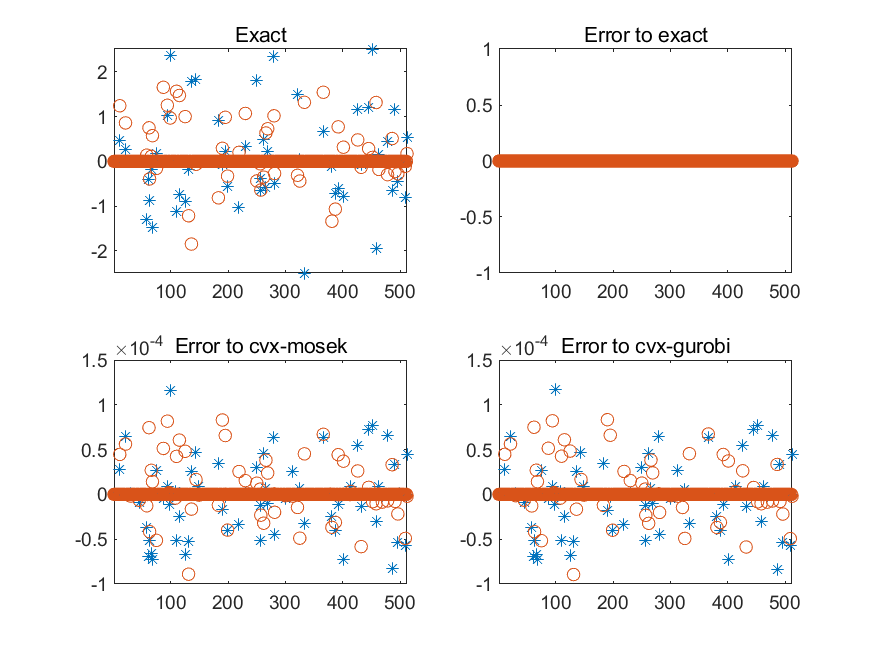
\includegraphics[width=0.7\textwidth]{C:/Users/沙柯岑/Desktop/大作业/figures/gl_exact.png} % 替换为实际路径
 	\caption{Exact solution and error analysis.}
 	\label{fig:error_analysis_exact}
 \end{figure}
 
 % CVX-Mosek
 \begin{figure}[htbp]
 	\centering
 	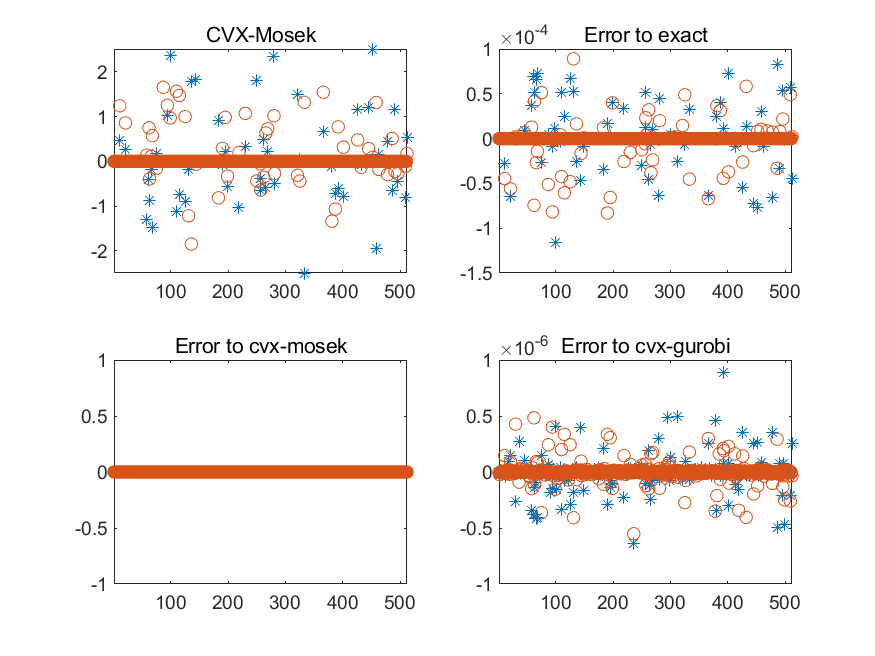
\includegraphics[width=0.8\textwidth]{C:/Users/沙柯岑/Desktop/大作业/figures/gl_cvx_mosek.png}
 	\caption{Error analysis for CVX-Mosek.}
 	\label{fig:error_analysis_cvx_mosek}
 \end{figure}
 
 % CVX-Gurobi
 \begin{figure}[htbp]
 	\centering
 	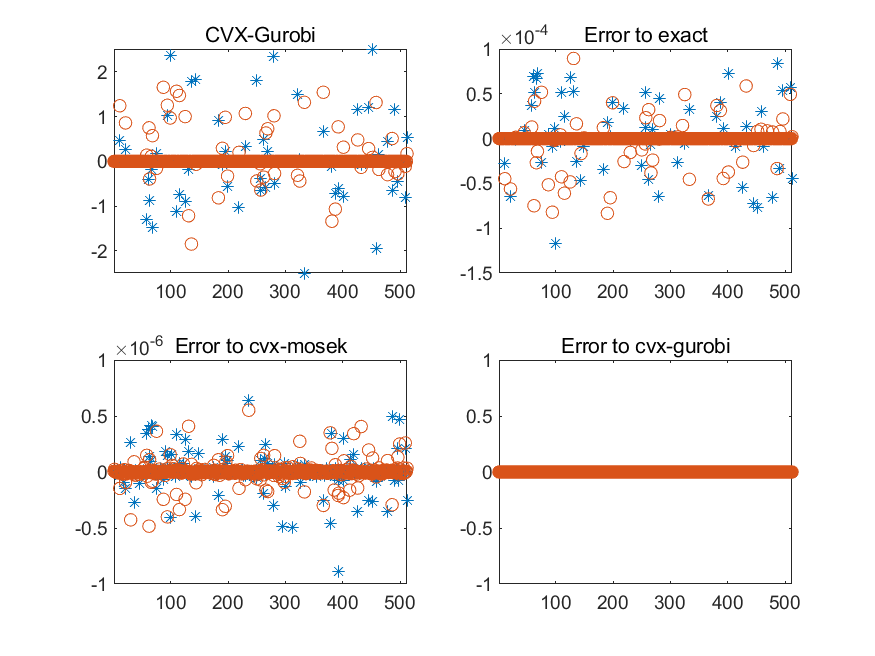
\includegraphics[width=0.8\textwidth]{C:/Users/沙柯岑/Desktop/大作业/figures/gl_cvx_gurobi.png}
 	\caption{Error analysis for CVX-Gurobi.}
 	\label{fig:error_analysis_cvx_gurobi}
 \end{figure}
 
 % Mosek
 \begin{figure}[htbp]
 	\centering
 	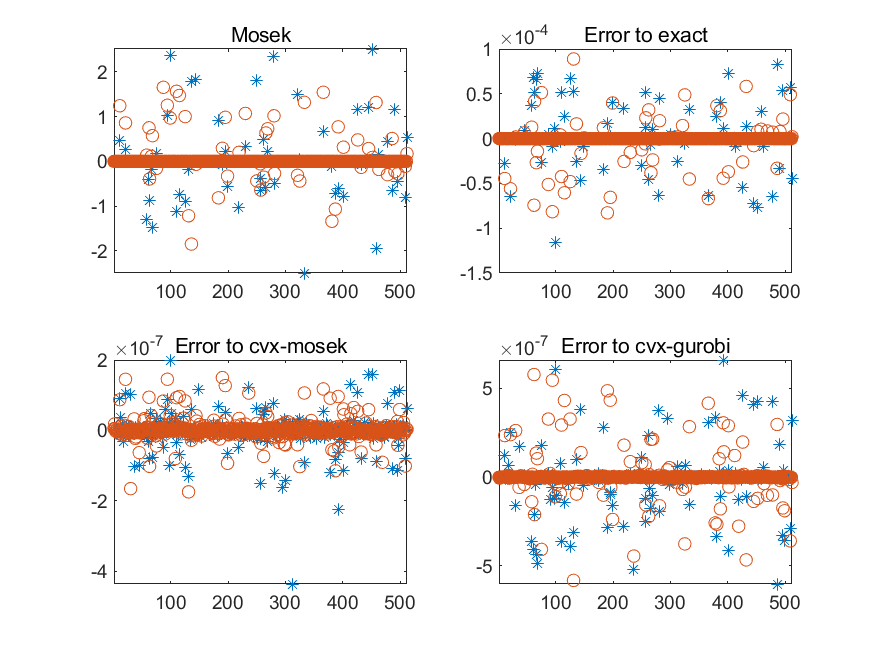
\includegraphics[width=0.8\textwidth]{C:/Users/沙柯岑/Desktop/大作业/figures/gl_mosek.png}
 	\caption{Error analysis for Mosek.}
 	\label{fig:error_analysis_mosek}
 \end{figure}
 
 % Gurobi
 \begin{figure}[htbp]
 	\centering
 	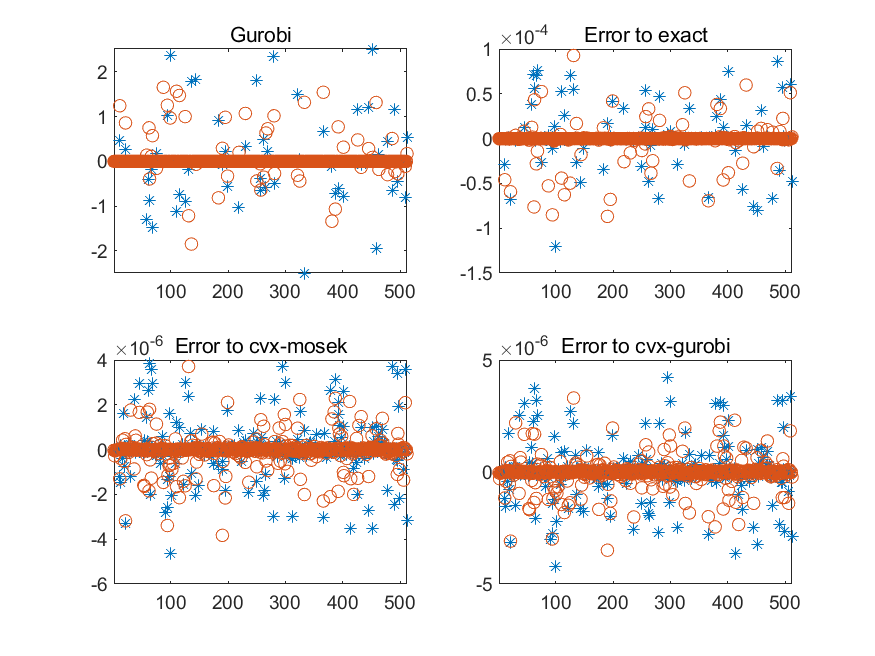
\includegraphics[width=0.8\textwidth]{C:/Users/沙柯岑/Desktop/大作业/figures/gl_gurobi.png}
 	\caption{Error analysis for Gurobi.}
 	\label{fig:error_analysis_gurobi}
 \end{figure}
 
 % SGD Primal
 \begin{figure}[htbp]
 	\centering
 	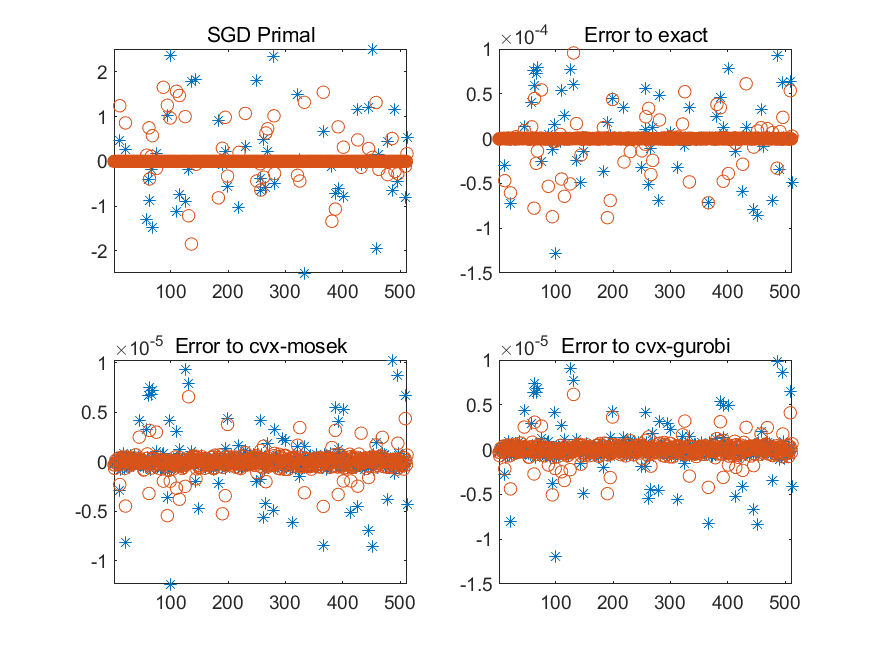
\includegraphics[width=0.8\textwidth]{C:/Users/沙柯岑/Desktop/大作业/figures/gl_SGD_Primal.png}
 	\caption{Error analysis for SGD Primal.}
 	\label{fig:error_analysis_sgd_primal}
 \end{figure}
 
 % GD Primal
 \begin{figure}[htbp]
 	\centering
 	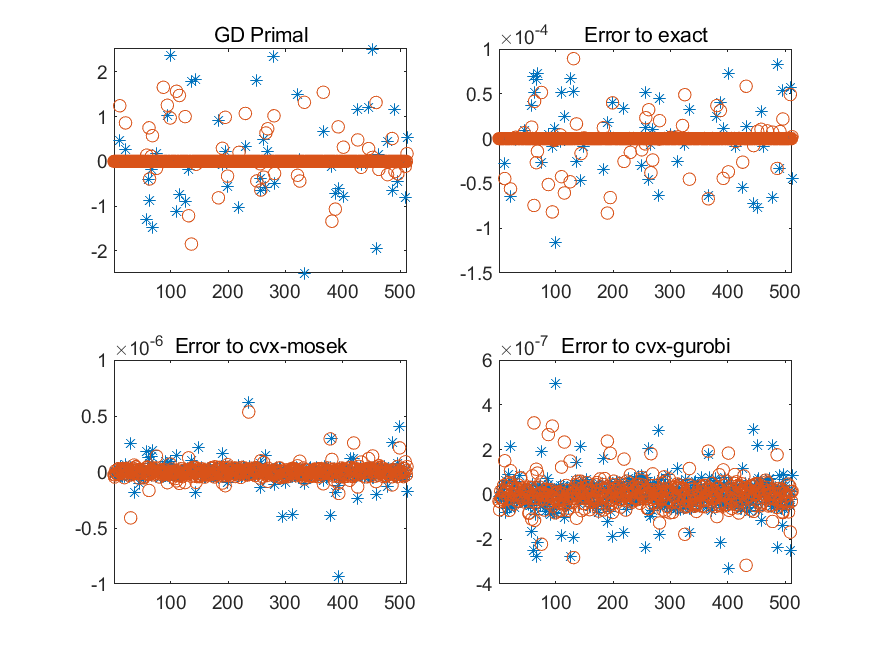
\includegraphics[width=0.8\textwidth]{C:/Users/沙柯岑/Desktop/大作业/figures/gl_GD_primal.png}
 	\caption{Error analysis for GD Primal.}
 	\label{fig:error_analysis_gd_primal}
 \end{figure}
 
 % FGD Primal
 \begin{figure}[htbp]
 	\centering
 	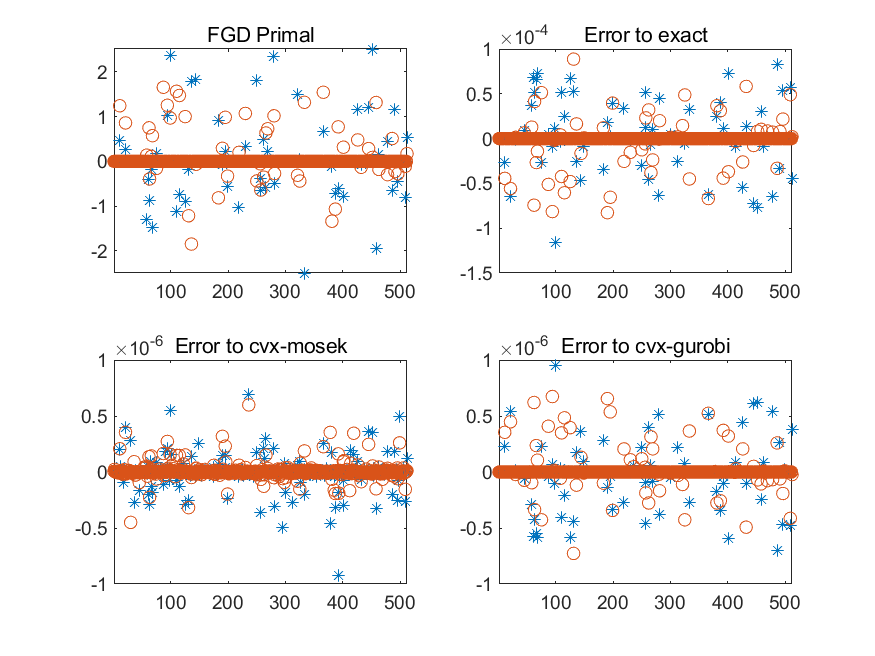
\includegraphics[width=0.8\textwidth]{C:/Users/沙柯岑/Desktop/大作业/figures/gl_FGD_primal.png}
 	\caption{Error analysis for FGD Primal.}
 	\label{fig:error_analysis_fgd_primal}
 \end{figure}
 
 % ProxGD Primal
 \begin{figure}[htbp]
 	\centering
 	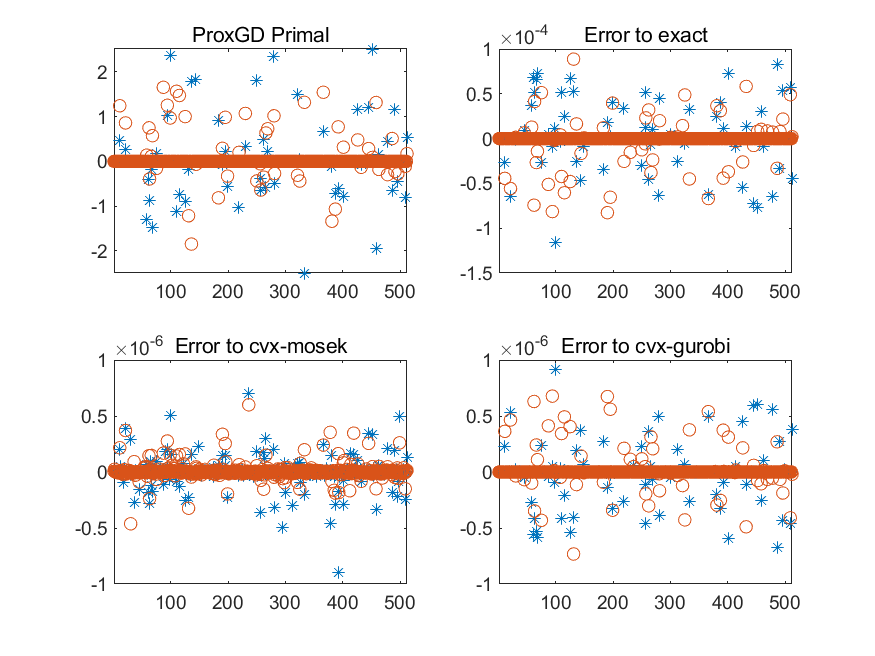
\includegraphics[width=0.8\textwidth]{C:/Users/沙柯岑/Desktop/大作业/figures/gl_ProxGD_primal.png}
 	\caption{Error analysis for ProxGD Primal.}
 	\label{fig:error_analysis_proxgd_primal}
 \end{figure}
 
 % FProxGD Primal
 \begin{figure}[htbp]
 	\centering
 	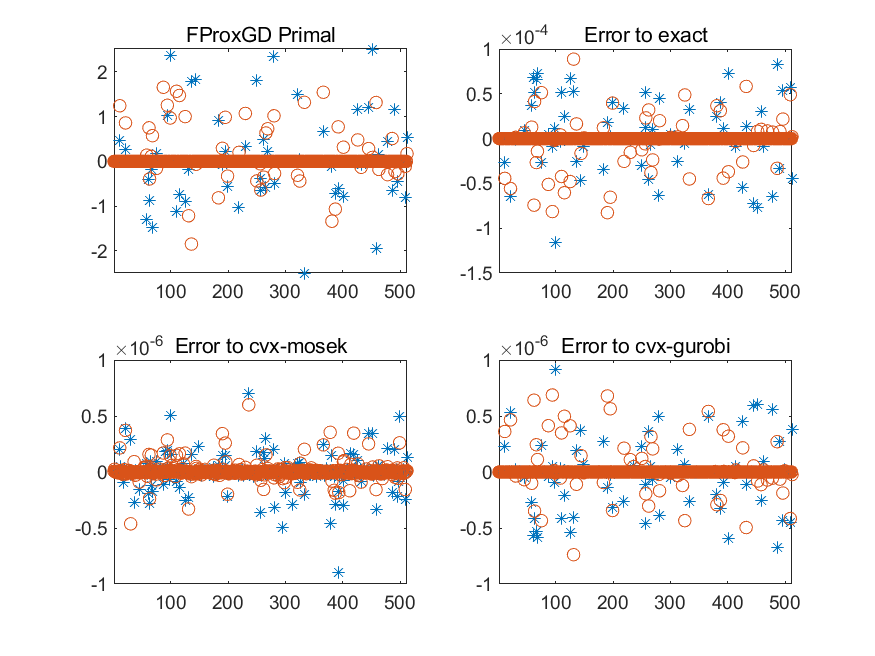
\includegraphics[width=0.8\textwidth]{C:/Users/沙柯岑/Desktop/大作业/figures/gl_FProxGD_primal.png}
 	\caption{Error analysis for FProxGD Primal.}
 	\label{fig:error_analysis_fproxgd_primal}
 \end{figure}
 
 % ALM Dual
 \begin{figure}[htbp]
 	\centering
 	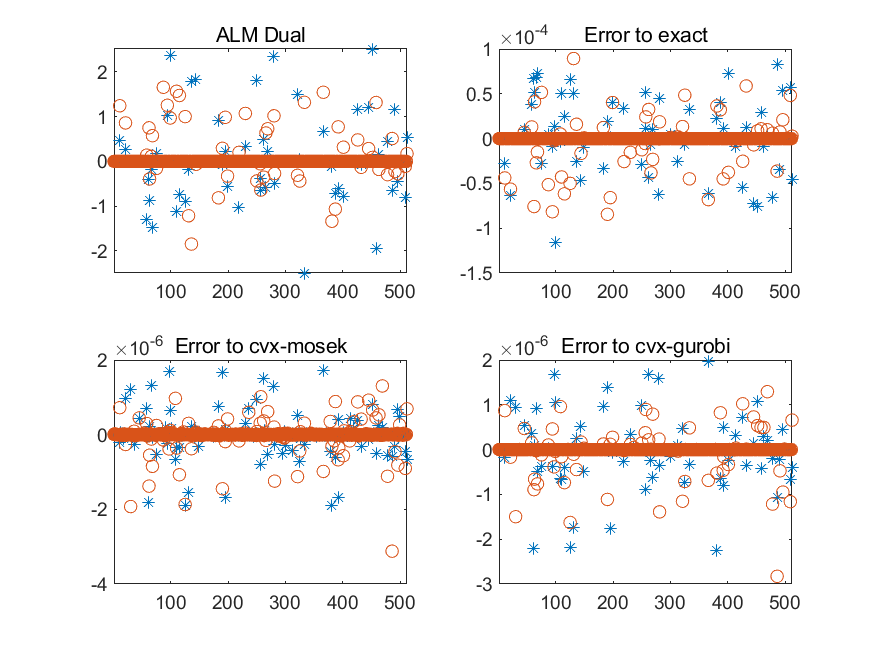
\includegraphics[width=0.8\textwidth]{C:/Users/沙柯岑/Desktop/大作业/figures/gl_ALM_dual.png}
 	\caption{Error analysis for ALM Dual.}
 	\label{fig:error_analysis_alm_dual}
 \end{figure}
 
 % ADMM Dual
 \begin{figure}[htbp]
 	\centering
 	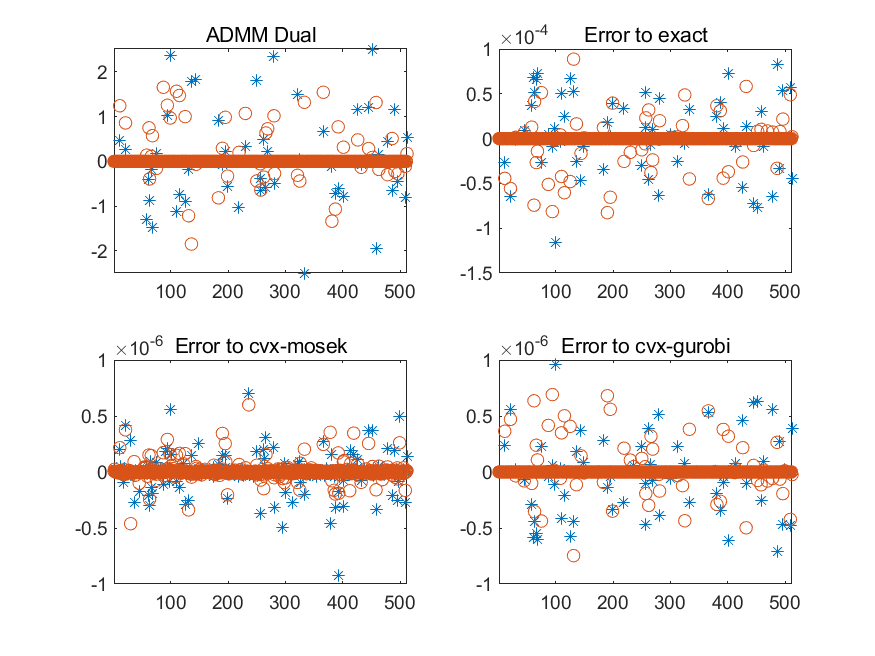
\includegraphics[width=0.8\textwidth]{C:/Users/沙柯岑/Desktop/大作业/figures/gl_ADMM_dual.png}
 	\caption{Error analysis for ADMM Dual.}
 	\label{fig:error_analysis_admm_dual}
 \end{figure}
 
 % ADMM Primal
 \begin{figure}[htbp]
 	\centering
 	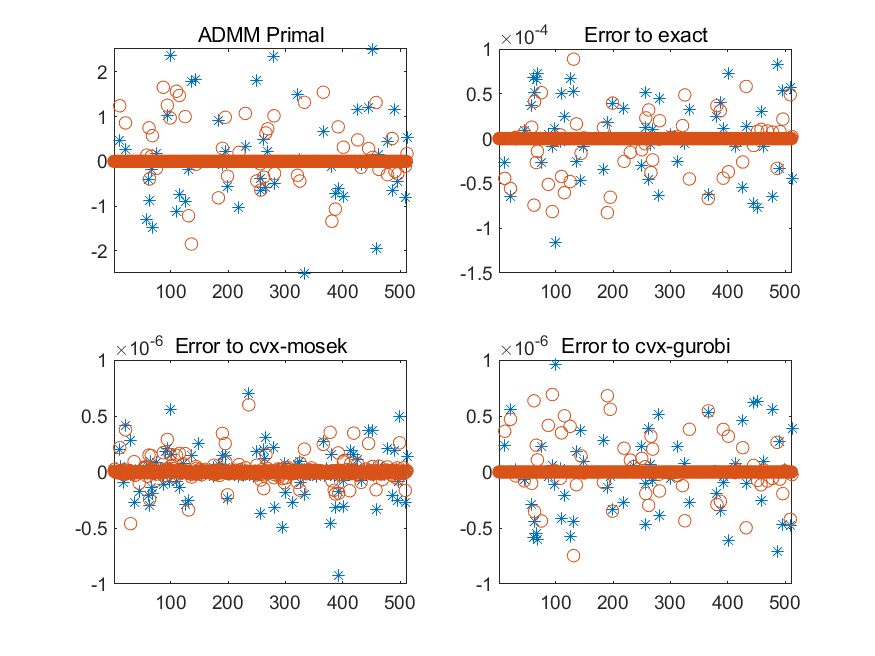
\includegraphics[width=0.8\textwidth]{C:/Users/沙柯岑/Desktop/大作业/figures/gl_ADMM_primal.png}
 	\caption{Error analysis for ADMM Primal.}
 	\label{fig:error_analysis_admm_primal}
 \end{figure}
\end{document}